\documentclass[border=10pt]{standalone}

\usepackage{tikz}
\usepackage{tikzsymbols}
\usetikzlibrary{calc,patterns,shapes.geometric}

\def\centerarc[#1](#2)(#3:#4:#5){\draw[#1] ($(#2)+({#5*cos(#3)},{#5*sin(#3)})$) arc (#3:#4:#5);}

\begin{document}
	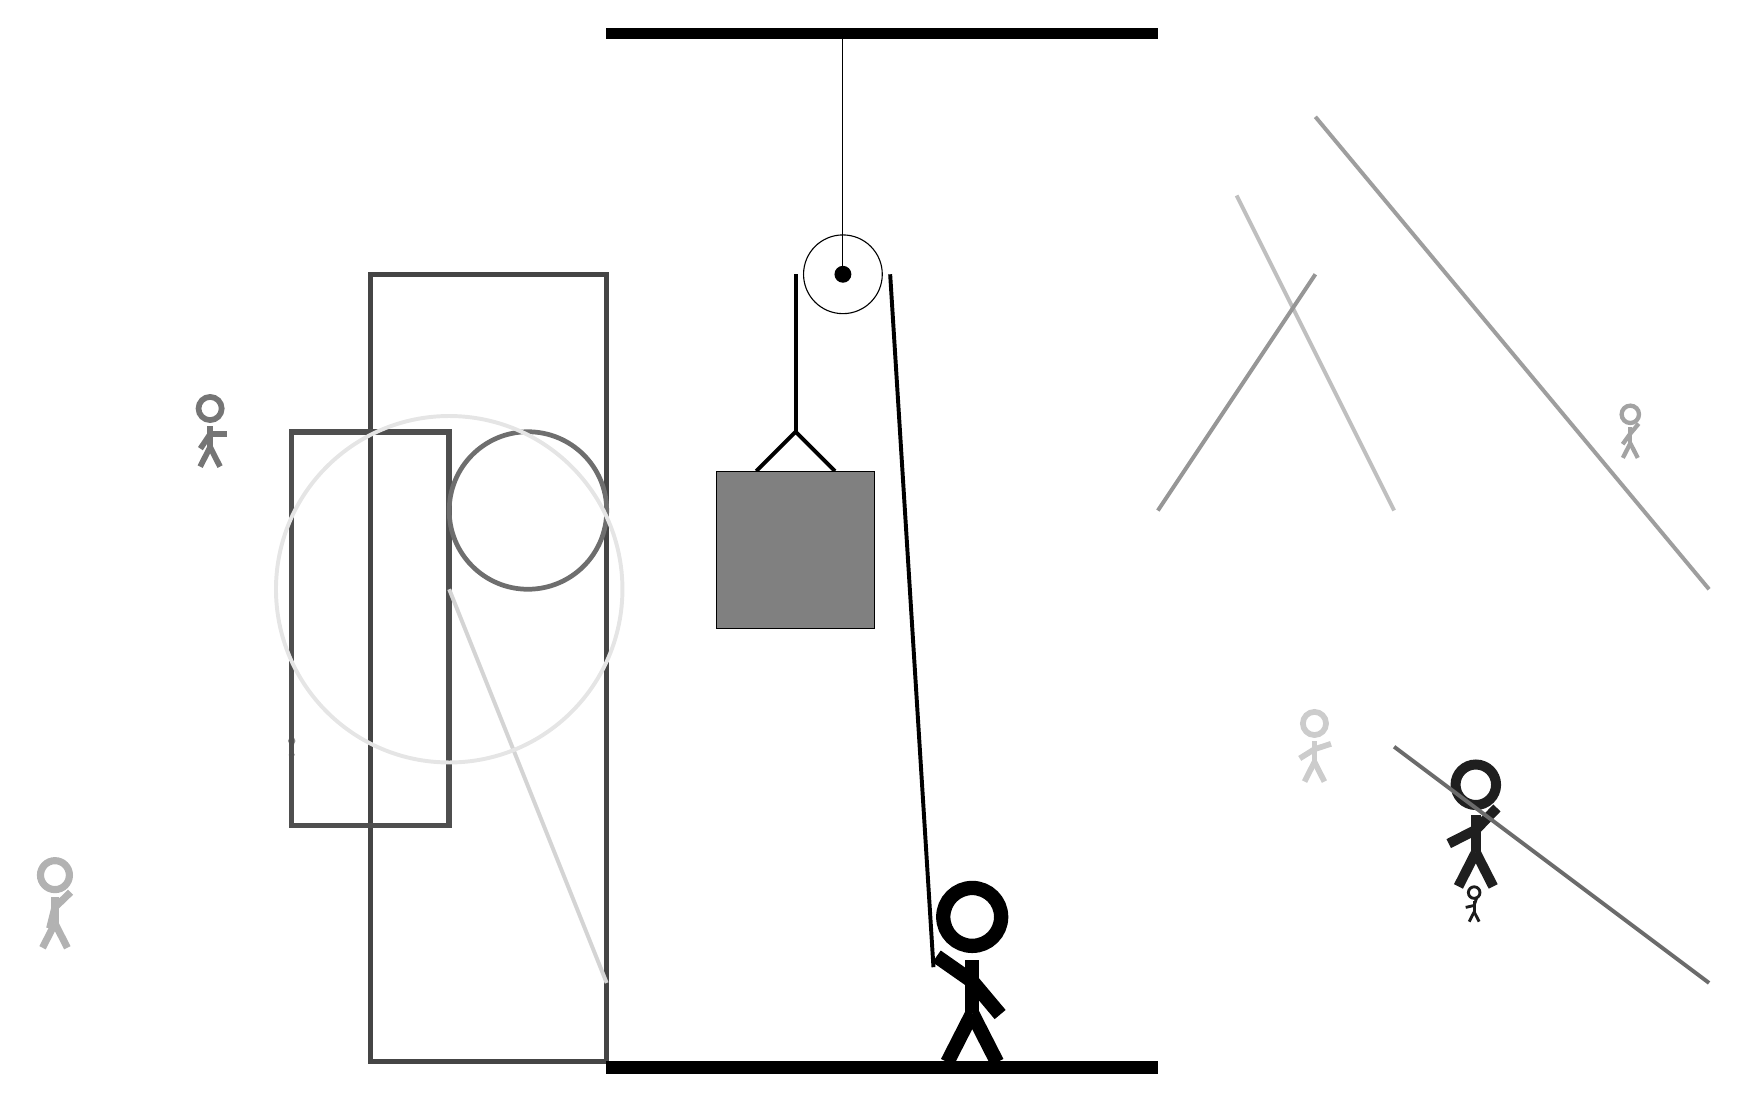
\begin{tikzpicture}
		%%%%% START %%%%%
		
		\draw[fill=black] (-2, 10) rectangle (5, 10.125);
		
		\draw (1, 7) circle (0.5);
		\draw[fill=black] (1, 7) circle (0.1);
		\draw (1, 10) -- (1, 7);
		
		\draw[line width=0.5mm] (-0.1, 4.5) -- (0.4, 5.0) -- (0.9, 4.5);
		\draw[fill=black!50] (-0.6, 4.5) rectangle (1.4, 2.5);
		
		\draw[line width=0.5mm] (0.4, 7) -- (0.4, 5.0);
		\centerarc[line width=0.5mm](1, 7)(0:180:0.6);
		\draw[line width=0.5mm](1.6, 7) -- (2.15, -1.8);
		
		\node[line width=0.5mm, color=black!30] at (-9, -1) {\Strichmaxerl[5][76][44]};
		
		\node[line width=0.7mm, color=black!46] at (-6, 1) {\Strichmaxerl[1][86][63]};
		\draw[line width=0.7mm, color=black!73] (-2, 7) rectangle (-5, -3);
		\node[line width=0.5mm, color=black!54] at (-7, 5) {\Strichmaxerl[4][56][0]};
		\draw[line width=0.7mm, color=black!69] (-4, 0) rectangle (-6, 5);
		\draw[line width=0.5mm, color=black!25](8, 4) -- (6, 8);
		\draw [line width=0.6mm, color=black!57](-3, 4) circle (1.0);
		
		\node[line width=0.6mm, color=black!36] at (11, 5) {\Strichmaxerl[3][54][50]};
		\node[line width=0.2mm, color=black!20] at (7, 1) {\Strichmaxerl[4][32][18]};
		\node[line width=0.5mm, color=black!88] at (9, 0) {\Strichmaxerl[7][27][46]};
		\draw[line width=0.5mm, color=black!41](7, 7) -- (5, 4);
		\draw[line width=0.5mm, color=black!17](-2, -2) -- (-4, 3);
		\draw [line width=0.5mm, color=black!10](-4, 3) circle (2.2);
		
		\draw[line width=0.5mm, color=black!38](7, 9) -- (12, 3);
		\draw[line width=0.5mm, color=black!58](8, 1) -- (12, -2);
		\node[line width=0.6mm, color=black!89] at (9, -1) {\Strichmaxerl[2][13][72]};
		
		
		\node at (2.6, -1.9) {\Strichmaxerl[10][-35][-50]};
		
		\draw[fill=black] (-2, -3) rectangle (5, -3.15);
		
		%%%%% END %%%%%
	\end{tikzpicture}
\end{document}